\documentclass[hyperref={pdfpagelabels=true}]{beamer}

\usepackage{lmodern}
%%%%%%%%%%%%%%%%%%%%%%%%%%%%%%%%%%%%%%%%%%%%%%%%%%%%%%%%%%%%%%%%%%%%%%%%%%%%%%%%%%%%%%%%%%%%%%%%%
%This work is licensed under a Creative Commons Attribution-ShareAlike 4.0 International License.
%
%You are free to:
%
%    Share — copy and redistribute the material in any medium or format
%    Adapt — remix, transform, and build upon the material
%    for any purpose, even commercially.
%
%    The licensor cannot revoke these freedoms as long as you follow the license terms.
%
%Attribution — You must give appropriate credit, provide a link to the license, and indicate if changes were made. You may do so in any reasonable manner, but not in any way that suggests the licensor endorses you or your use.
%
%ShareAlike — If you remix, transform, or build upon the material, you must distribute your contributions under the same license as the original. 
%
%%%%%%%%%%%%%%%%%%%%%%%%%%%%%%%%%%%%%%%%%%%%%%%%%%%%%%%%%%%%%%%%%%%%%%%%%%%%%%%%%%%%%%%%%%%%%%%%%
\definecolor{dred}{rgb}{0.647059, 0.164706, 0.164706}
\definecolor{dgreen}{rgb}{0., 0.545098, 0.545098}
\usecolortheme[named=dgreen]{structure}

\title{Analysing GeoLocated Data from Social Media}
\subtitle{with QGIS}
\author{Joana Sim\~{o}es} 

\author[shortname]{Joana Sim\~{o}es \inst{1}}
\institute[shortinst]{\inst{1} Bdigital, CASA, CICS.NOVA}

%\date{\today} 
%\titlegraphic{\includegraphics[width=.35\textwidth]{bigdata2.png}}
 
\usepackage{beamerthemeshadow}
%\usepackage{beamerthemesplit}
\usepackage{listings}

\newcommand{\soooo}{H$_2$SO$_4$}

%fdl stuff
\usepackage{hyperref}
\hypersetup{colorlinks, 
           citecolor=black,
           filecolor=black,
           linkcolor=black,
           urlcolor=black,
           bookmarksopen=true,
           pdftex}

\hfuzz = .6pt % avoid black boxes

\lstset{language=SQL}

\begin{document}
\setbeamertemplate{footline}[page number]
\setbeamertemplate{navigation symbols}{}
\begin{frame}
%\titlepage

\begin{titlepage}
\centering{ 
  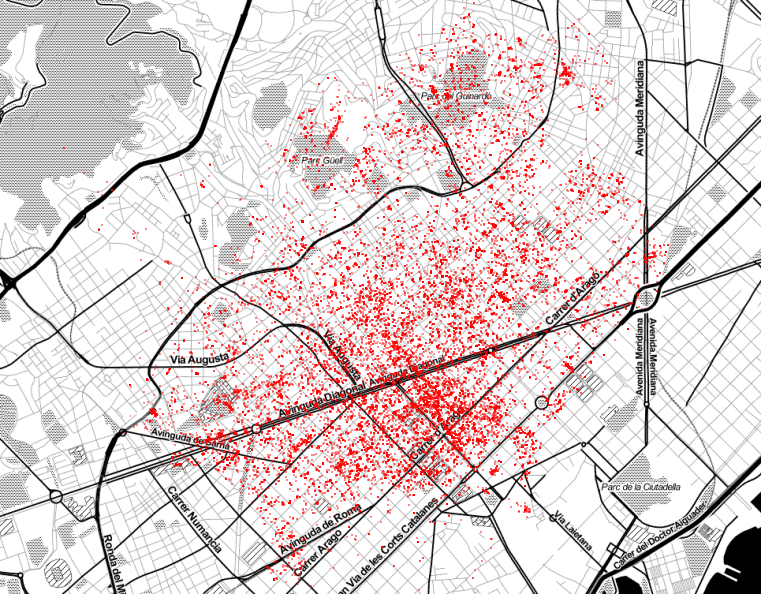
\includegraphics[height=50px]{raw_data.png}    
  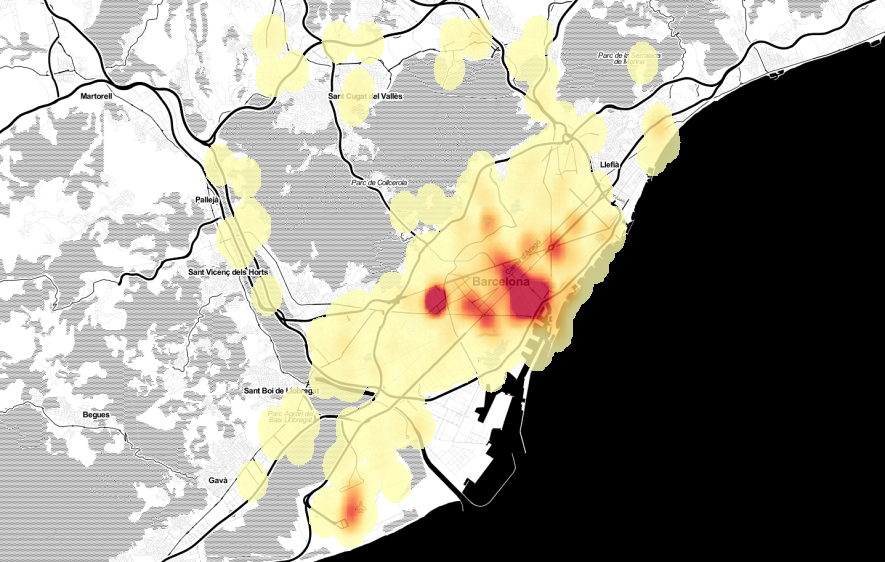
\includegraphics[height=50px]{cover3.png}  
  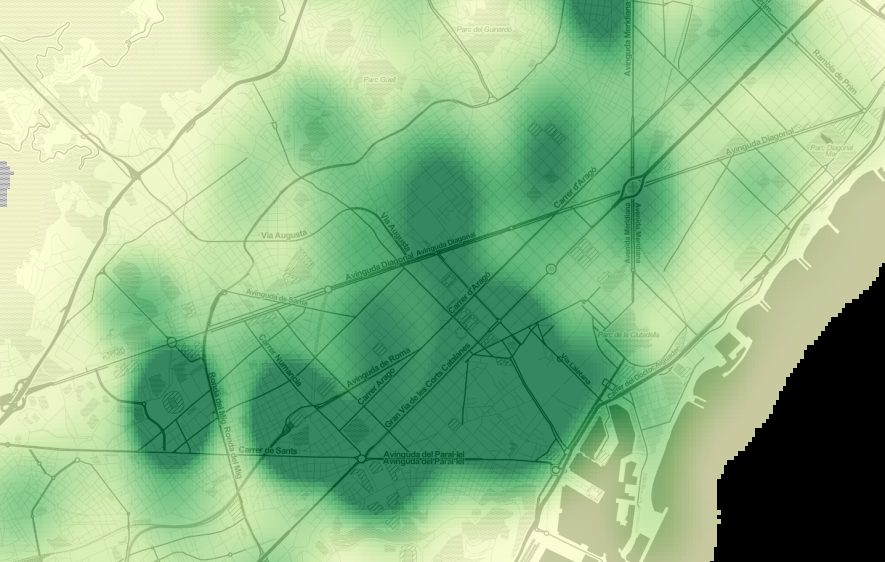
\includegraphics[height=50px]{cover2.png}    
  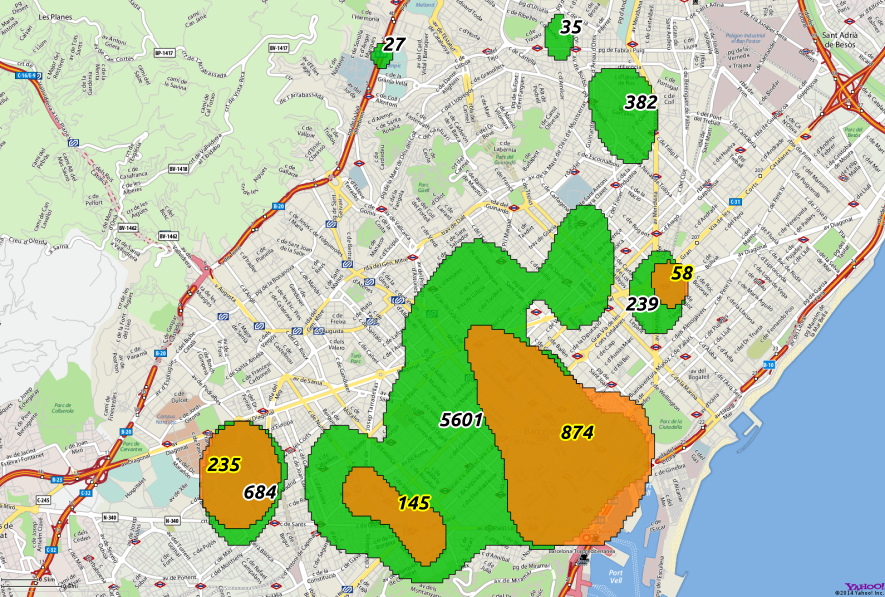
\includegraphics[height=50px]{cover1.png}  
}
\end{titlepage}

\end{frame} 
  
 
\begin{frame}
\frametitle{Table of Contents}
%\tiny{
\tableofcontents%}
\end{frame}

\section{Introduction} 
\begin{frame}
\frametitle{What do we want to do?}

\begin{itemize}
  \item<1->Nowadays social media is a major source for information sharing. In some cases the user also shares some attributes, such as \textbf{geolocation}. By using this information as a proxy for human presence, and with the adequate methods, we are able to provide powerful representations of the distribution of social media users within the territory.
  \item<2->Due to its willingness in sharing data, Twitter has been a prime \textit{playground}, for researchers and practitioners around the world.
  \item<3->The objective of this workshop is to provide a workflow for enhancing the visualization of geolocated Tweets.
  \end{itemize}

\end{frame}

\begin{frame}
\frametitle{How are we going to do it?}

\begin{itemize}
  \item<2->Pull data stored in a NoSQL database.
  \item<3->Create an Heatmap expressing Tweet density.
  \item<4->Produce clusters from the heatmap.
  \item<5->Produce a 3D visualization, on a webpage.  
\end{itemize}

\end{frame}

\begin{frame}
\frametitle{Objective}
\begin{columns}
  \begin{column}{0.5\textwidth}
      \begin{figure}  
	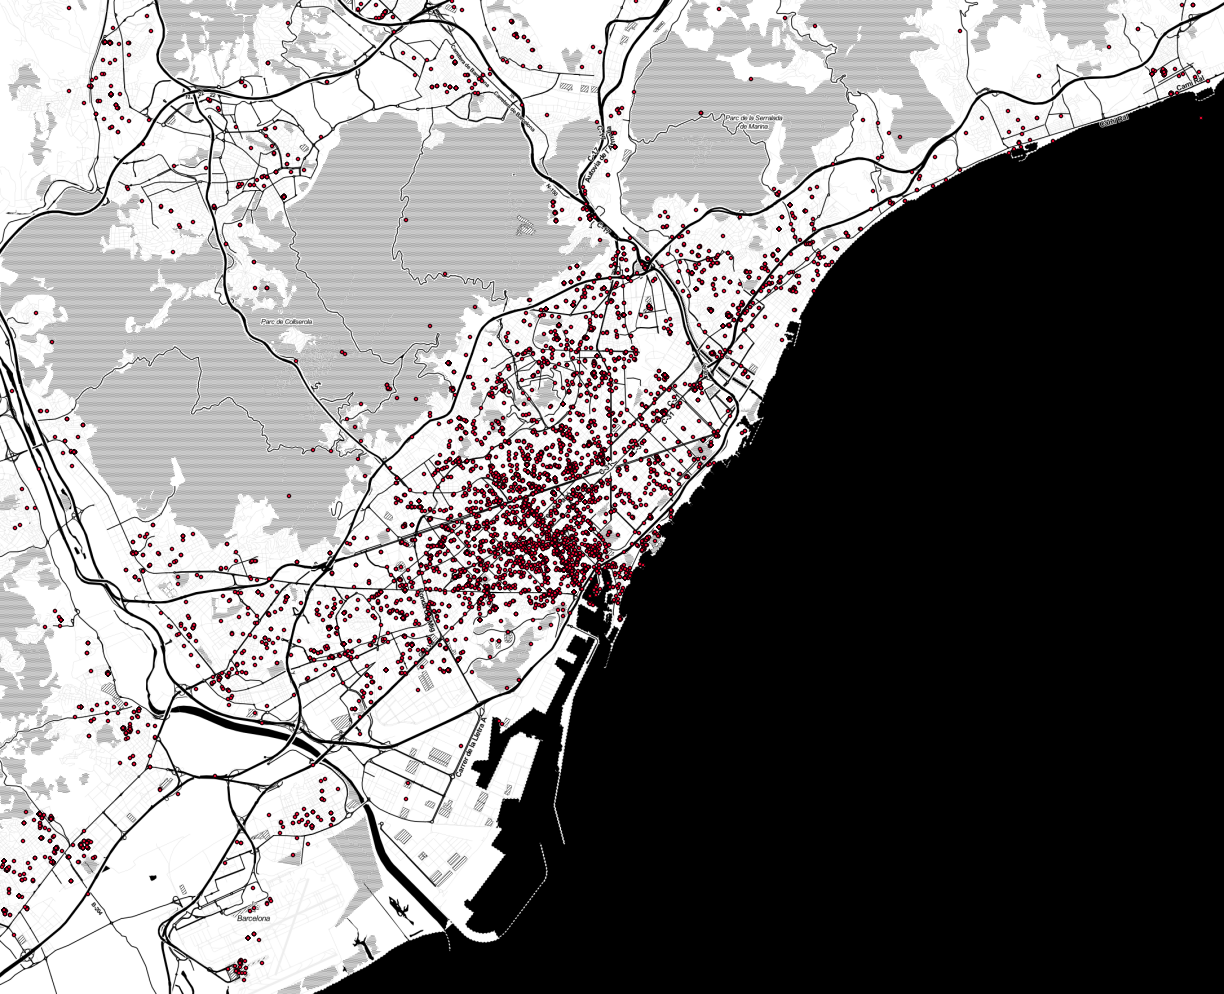
\includegraphics[width=\textwidth]{tweets_cat.png}\\
       \end{figure}    
    \tiny{Before: Raw tweets}         
  \end{column}
  \begin{column}{0.5\textwidth}
      \begin{figure}  
	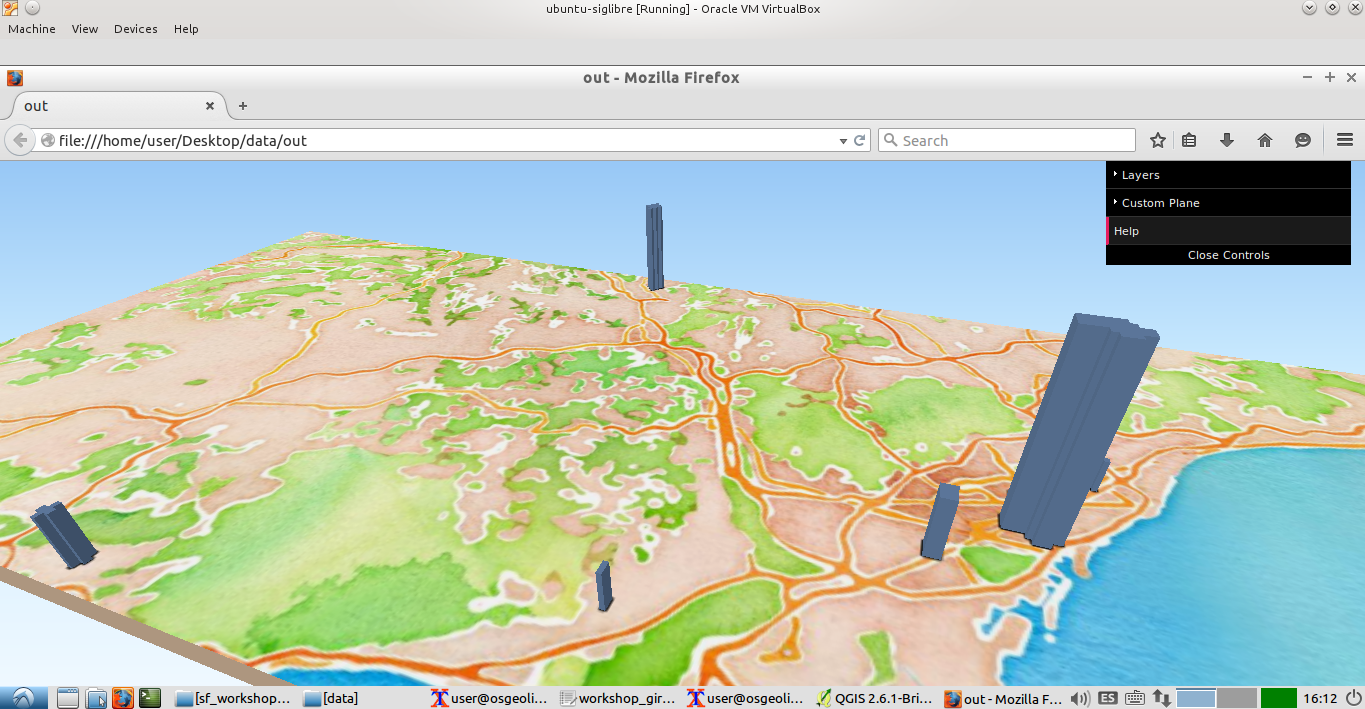
\includegraphics[width=\textwidth]{final.png}\\
       \end{figure}  
    \tiny{After: 3D visualization of the clusters of tweets}  
  \end{column}  
\end{columns}
\end{frame}

\begin{frame}
\frametitle{Stack}

\begin{columns}
  \begin{column}{0.5\textwidth}
\begin{itemize}
  \item MongoDB
  \item QGIS + Python Plugins
  \begin{itemize}
    \item<2-> Heatmap
    \item<3-> OpenLayers
    \item<4-> Qgis2threejs    
  \end{itemize}    
\end{itemize}
  \end{column}
  \begin{column}{0.5\textwidth}
      \begin{figure}  
	
\includegraphics[width=0.3\textwidth]{mongodb_logo.png}\\
       \end{figure}  
      \begin{figure}  
	
\includegraphics[width=0.3\textwidth]{qgis_logo.jpg}\\
       \end{figure}         
  \end{column}  
\end{columns}



\end{frame}

\begin{frame}
\frametitle{Approach}
This will be a hands-on workshop.\small{ 
\begin{itemize}
  \item<2-> People will partner up in small teams.
  \item<3-> I will introduce each one of the micro-tasks, and I will do it while you watch.
  \item<4-> Then I will provide help to everyone who needs it to complete the task.
  \item<5-> \textbf{For the impatient:} If you don't want to wait for everyone to complete, you may attempt to complet the exercises on your own ;-) View the complete presentation here: \url{http://tinyurl.com/pltwtc2}
  \item<6-> \textbf{For the guru:} If you have finished everything and are bored, you may want to read some of the links, on the last page, or help your colleagues to complete the tasks ;-)
\end{itemize}}
\end{frame}

\section{Getting the Tweets Coordinates} 
\begin{frame}
\frametitle{Twitter Data}

\begin{columns}
  \begin{column}{0.5\textwidth}\small{ 
    \begin{itemize}
      \item<1->Users on Twitter generate over 400 million tweets everyday.
      \item<1->A proportion of these tweets is available to researchers and practitioners through public APIs, free of any charges.
      \item<2->Approximately 1\% of all Tweets published on Twitter are geolocated.%Users can optionally choose to provide location information for the Tweets they publish. gps still 4 million everyday
      \end{itemize}  }
  \end{column}
  \begin{column}{0.5\textwidth}
      \begin{figure}  
	
\includegraphics[width=\textwidth]{love.jpg}\\
       \end{figure}  
    \tiny{Why we love Twitter}  
  \end{column}  
\end{columns}
\end{frame}

\begin{frame}
\frametitle{Twitter APIs}

\begin{itemize}
  \item<2->REST APIs. %use pull strategy for data retrieval.To collect information a user must explicitly request it
  \item<3->StreamAPIs. %provides a continuous stream of public information from Twitter. These APIs use the push strategy for data retrieval.
  \begin{itemize}  
    \item<4->User streams. %These are single-user streams, with to all the Tweets of auser
    \item<5->Site streams. % These are multi-user streams and intended for applicationswhich access Tweets from multiple users
    \item<6->Public Streams. %These are streams containing the public tweets on Twitter    
  \end{itemize}  
  \item<7->These APIs are accessed only via authenticated requests (OAuth).% each request must be signed with valid Twitter user credentials  
  \item<8->Access to APIs is also limited to a specific number of requests within a time window (rate limit). %apply to user and app. 15 mining
  \item<9->Responses from Twitter are in JSON format.
\end{itemize}  

\end{frame}

\begin{frame}
\frametitle{JSON in a Nutshell}

\begin{columns}
  \begin{column}{0.5\textwidth}
    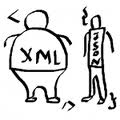
\includegraphics[width=0.5\textwidth]{json2.jpg}  
  \end{column}
  \begin{column}{0.5\textwidth}
    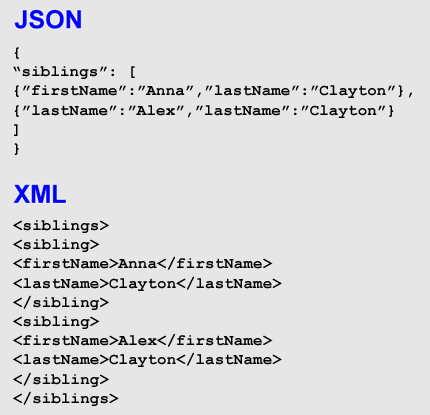
\includegraphics[width=\textwidth]{json.png}    
  \end{column}  
\end{columns}

\end{frame}

\begin{frame}
\frametitle{Mongo loves JSON}
\begin{itemize}
  \item<1->NoSQL Database.
  \item<1->Document-Oriented Storage.%MongoDB stores its data in JSON-style objects. This makes it very easy to store raw documents from Twitter’s APIs
\end{itemize}
    \begin{figure}  
      
\includegraphics[width=0.5\textwidth]{mongo.png}  
    \end{figure}  
\end{frame}


\begin{frame}
\frametitle{Hands-on}
\begin{itemize}
  \item<1->Objective: Connect to the tweets database and view one record.
  \item<2->Tool: Mongodb command line client.
  \item<2->Database properties:
  \begin{itemize}  
    \item<2->host: 54.72.72.228 (on aws).
    \item<2->database: tweets\_workshop
    \item<2->username: workshop
    \item<2->password: geohipster
    \item<2->collection: tweets    
  \end{itemize}  
  \item<2->Reference: \url{http://docs.mongodb.org/manual/\#}.
  \item<3-> \textit{mongo --host 54.72.72.228 tweets\_workshop -u workshop -p geohipster}
  \item<3->\textit{db.tweets.find().limit( 1 )}  
\end{itemize}  
\end{frame}

\begin{frame}
\frametitle{Hands-on (cont.)}
\begin{itemize}
  \item<1->Objective: Export tweets coordinates into a csv file.
  \item<2->Take notice of the long, lat fields.
  \item<2->Exit the client.  
  \item<2->Use mongoexport to write the values on a text file.    
  \item<2->Reference: \url{http://docs.mongodb.org/manual/core/import-export/}.
  \item<3->\textit{ mongoexport --host  54.72.72.228 -u workshop -p geohipster --db tweets\_workshop --collection tweets --csv --out out\_tweets.csv --fields geoLocation.longitude,geoLocation.latitude --query  '{geoLocation: {\$ne: null}}'}
  \item<3->View the exported file:e.g.: \textit{cat /tmp/out/out\_tweets.csv}  
\end{itemize}  
\end{frame}

\section{Importing the Tweets into QGIS} 
\begin{frame}
\frametitle{QGIS}
QGIS is a Free and Open-Source GIS System:
    \begin{itemize}
      \item<2->Cross-platform (Windows, Mac, Linux and Android).
      \item<3->Easy to use.
      \item<4->Great community support.
      \item<5->Latest version has been translated into 46 languages.
      \end{itemize}
      
    \begin{figure}  
      
\includegraphics[width=\textwidth]{qgis.png}\\
      \end{figure}  
       
\end{frame}

\begin{frame}
\frametitle{Bug Affecting the Heatmap Plugin}
      
  \begin{figure}  
    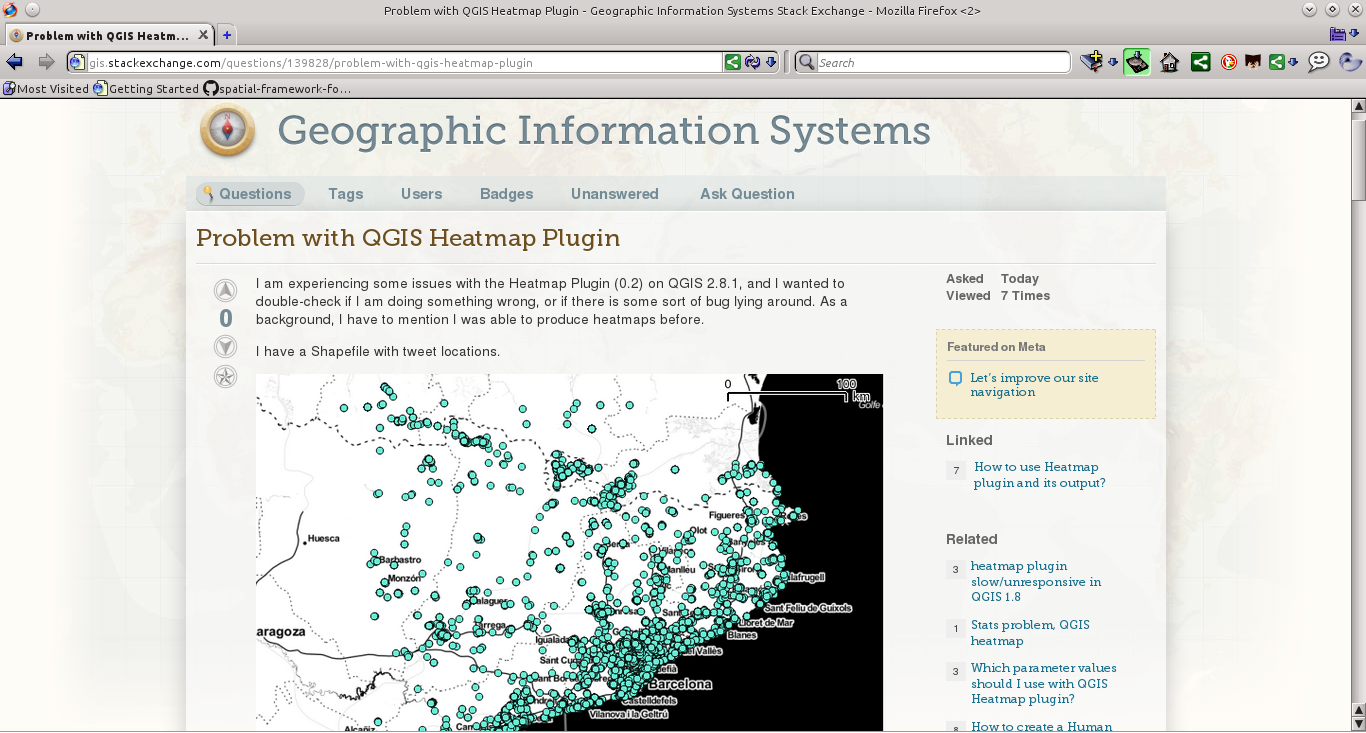
\includegraphics[width=\textwidth]{bug.png}\\
    \end{figure}  
       
\end{frame}

\begin{frame}
\frametitle{There is a Plugin for Everything}

\begin{itemize}
  \item<1->The core of QGIS is extended through user-submited Python plugins.
  \item<3->Plugins can be easily installed through the plugin manager.%there are plugins forinput, output,processing, etc
  \item<4->In this workshop we will use three plugins (one is already installed).
\end{itemize}
      
  \begin{figure}  
    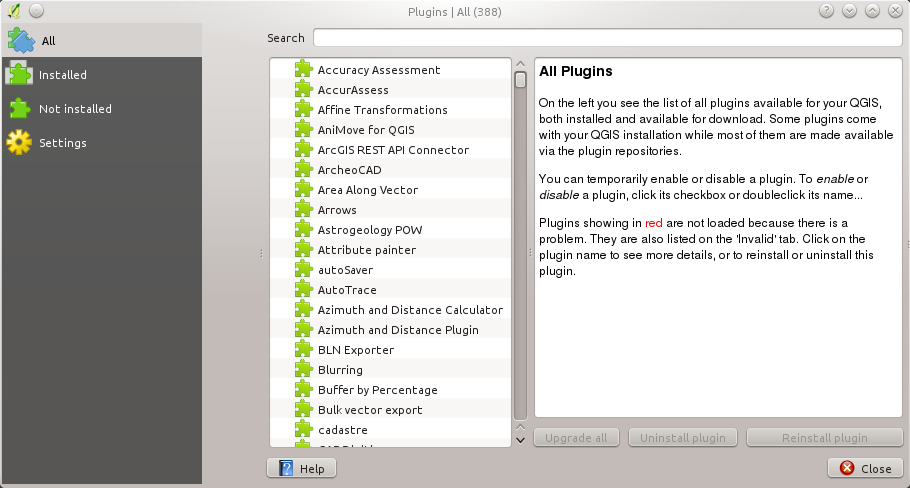
\includegraphics[width=0.6\textwidth]{plugins.png}\\
    \end{figure}         
\end{frame}

\begin{frame}
\frametitle{Isn't there a Plugin to connect to MongoDB?}
\begin{itemize}
  \item<1->A plugin was written in 2011.
  \item<3->There seemed to be some issues with it, and sadly it hasn't be ported to the latest versions of QGIS.
  \item<4->The project appears to be now dead.
  \item<5->The community would really welcome a new attempt for a mongoDB connector on QGIS.  
\end{itemize}      
  \begin{figure}  
      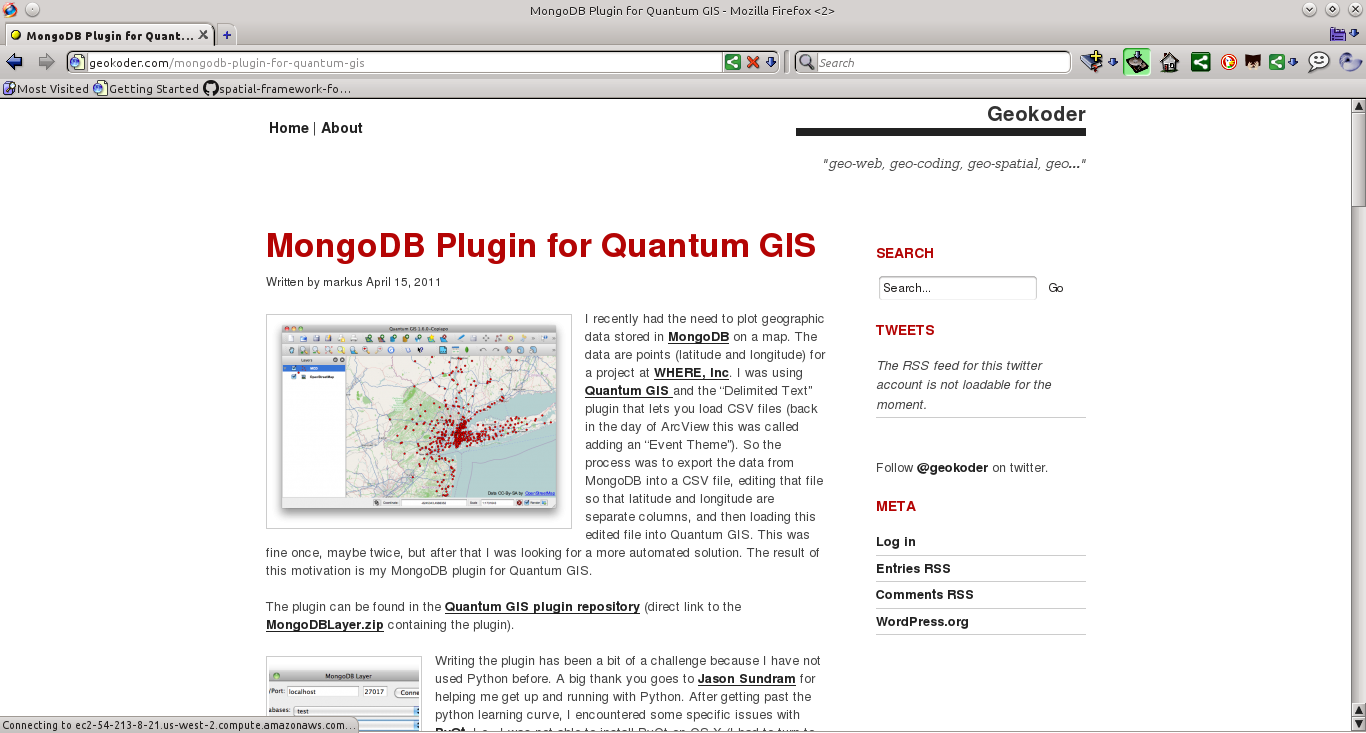
\includegraphics[width=0.6\textwidth]{mongodbplugin.png}\\
    \end{figure}         
\end{frame}

\begin{frame}
\frametitle{Hands-on}
\begin{itemize}
  \item<1->Objective: Display the tweets coordinates in QGIS, with background map.
  \item<1->Tool: QGIS + OpenLayers plugin.
  \item<1->Steps: \small{  
  \begin{itemize}
    \item<2->Start QGIS and create a project.  
    \item<2->Download and enable the \textit{OpenLayers} plugin (Plugins$\rightarrow$Manage and Install Plugins).
    \item<2->Choose a background map (e.g.: OSM, Bing Maps, etc).
    \item<2->Import the JSON file, using the Text Layer Importer (Layer$\rightarrow$Add Layer$\rightarrow$Add Delimited Text Layer).
  \end{itemize}   }
\end{itemize}  

  \begin{figure}  
      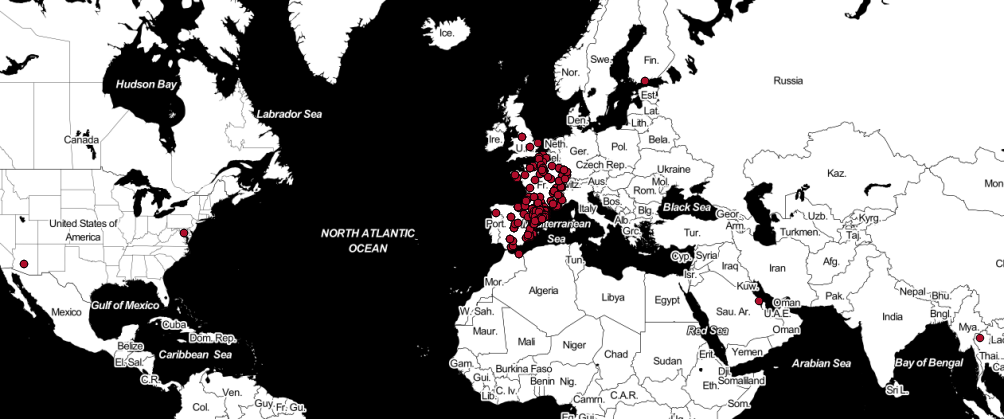
\includegraphics[width=0.4\textwidth]{import.png}\\
    \end{figure}         

\end{frame}

\begin{frame}
\frametitle{Hands-on (cont.)}
\begin{itemize}
  \item<1->Objective: Save the tweets from the region of Catalunya, in a Shapefile.
  \item<1->Steps:  
  \begin{itemize}
    \item<2->Zoom into the desired location using the zoom tool (View$\rightarrow$Zoom in) .  
    \item<2->Select the visible points using the select tool.
    \item<2->Save the selected features in a Shapefile.
    \begin{itemize}
      \item<2->Pay attention to the crs.
      \item<2->Make sure you save \textbf{only} the selected features.      
    \end{itemize}    
  \end{itemize}    
\end{itemize}  

  \begin{figure}  
      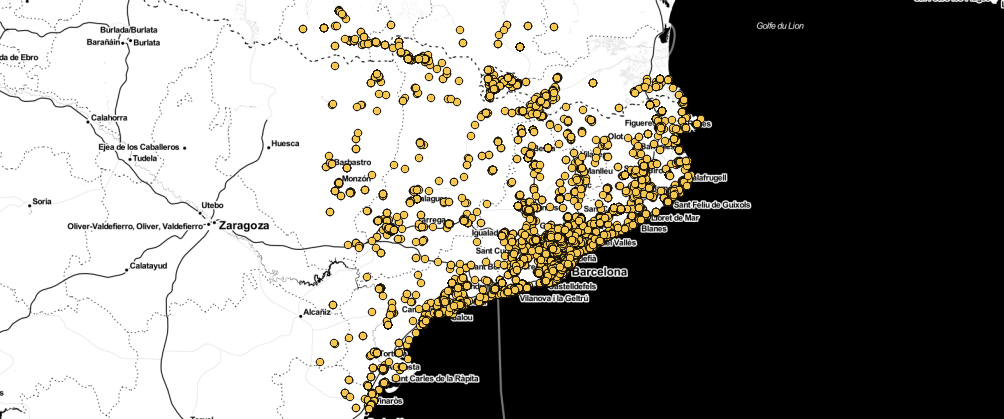
\includegraphics[width=0.6\textwidth]{sel_tweets.png}\\
    \end{figure}         
\end{frame}

\section{Creating an Heatmap} 
\begin{frame}
\frametitle{Heatmaps}

Heatmaps enhance the visualization of the density distribution of a phenomena (e.g.: crime, accidents, tweets).
\begin{columns}
  \begin{column}{0.5\textwidth}
    \begin{itemize}
	  \item<2->The \textit{heat} in the term refers to the concentration of the geographic entity within any given spot.
	  \item<3->Sometimes they are referred as \textit{hot spot} mapping or \textit{clustering}.
	  \item<4->They are great tools to detect spatial patterns.
    \end{itemize}
  \end{column}
  \begin{column}{0.5\textwidth}
    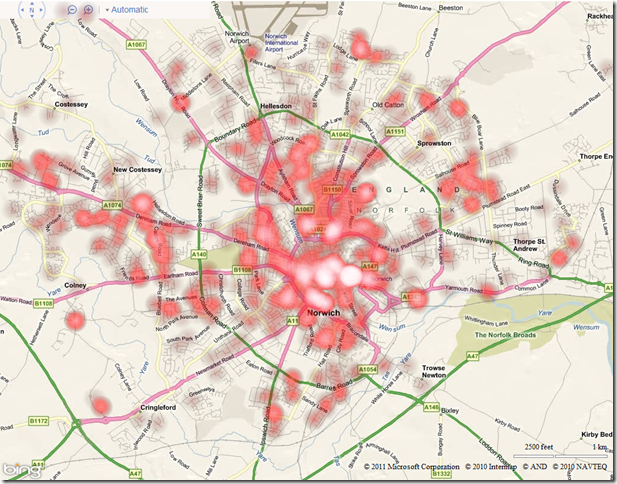
\includegraphics[width=\textwidth]{heatmap_crime.png}    
  \end{column}  
\end{columns}
\end{frame}

\begin{frame}
\frametitle{Heatmaps (cont.)}

\begin{itemize}
      \item<1->Creating heatmaps involves interpolating discrete points to create a continuous surface known as a \textbf{density surface}. 
      \item<2->There are three key parameters involved in this calculation:
  \begin{itemize}
	\item<3->Cell size of the output raster file.%resolution: a small cell size will result in a smoother surface, but it will result in a larger file.
	\item<3->Bandwidth or search radius.% the area around each cell the GIS software will factor into the density calculation. too small will pick up only local patterns, and too large will generalize too much.
	\item<3->Interpolation algorithm.%anything from count features within a search radius to IDW, 
	
  \end{itemize}
\end{itemize}
\end{frame}


\begin{frame}
\frametitle{Hands-on}
\begin{itemize}
  \item<1->Objective: Create heatmap depicting tweet density.
  \item<1->Tool: QGIS + Heatmap plugin.
  \item<1->Steps:  
  \begin{itemize}
    \item<2->Ensure the heatmap plugin is enabled.  
    \item<2->Create the heatmap using the plugin (Raster$\rightarrow$Heatmap).
    \item<2->Pay special attention to the following parameters:    
    \begin{itemize}
      \item<3->Radius: search radius in meters.
      \item<3->Rows and columns: cell size of the output raster.
      \item<3->Kernel shape: QGIS uses one of the following decay algorithms.      
    \end{itemize}        
    \item<4->Costumize the color scheme, by right clicking the layer and choosing properties.
  \end{itemize}    
\end{itemize}  
\end{frame}

\begin{frame}
\frametitle{Hands-on (cont.)}
%pictures of heatmaps

\begin{itemize}  
    \item<1->Suggestion: try different combinations of parameters and different visualizations.    
    \item<1->Tip: Use the identify tool to ensure the maximum is being correctly picked up.
\end{itemize}  

  \begin{figure}  
      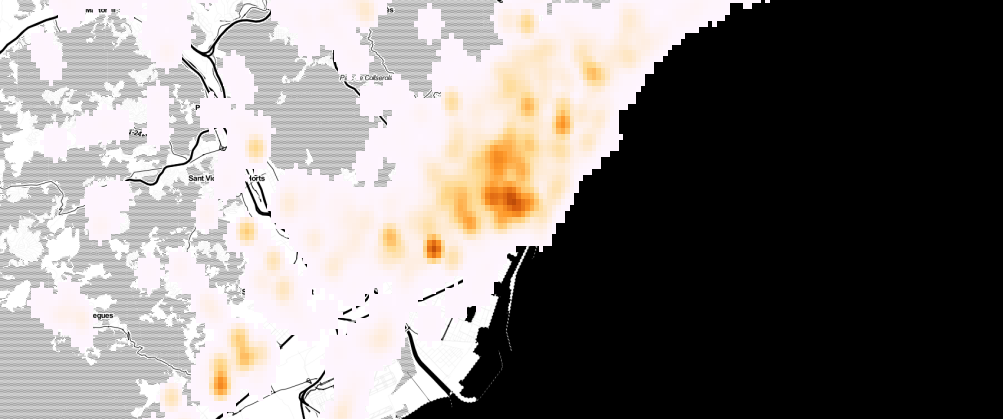
\includegraphics[width=\textwidth]{heatmap1.png}\\
    \end{figure}         

\end{frame}

\section{Creating Clusters} 
\begin{frame}
\frametitle{Clustering}
\small{ 
    \begin{itemize}
      \item<1->It is a descriptive data mining technique, often used for dimensionality reduction.
      \item<2->It corresponds to a family of unsupervised machine learning algorithms.      
      \item<3->It groups a set of objects in such a way that objects in the same group are more similar to each other, than to object in other groups.
      \item<4->Density based clusters are separated from each other by contiguous regions of low density of objects.
    \end{itemize}    
}
  \begin{figure}  
      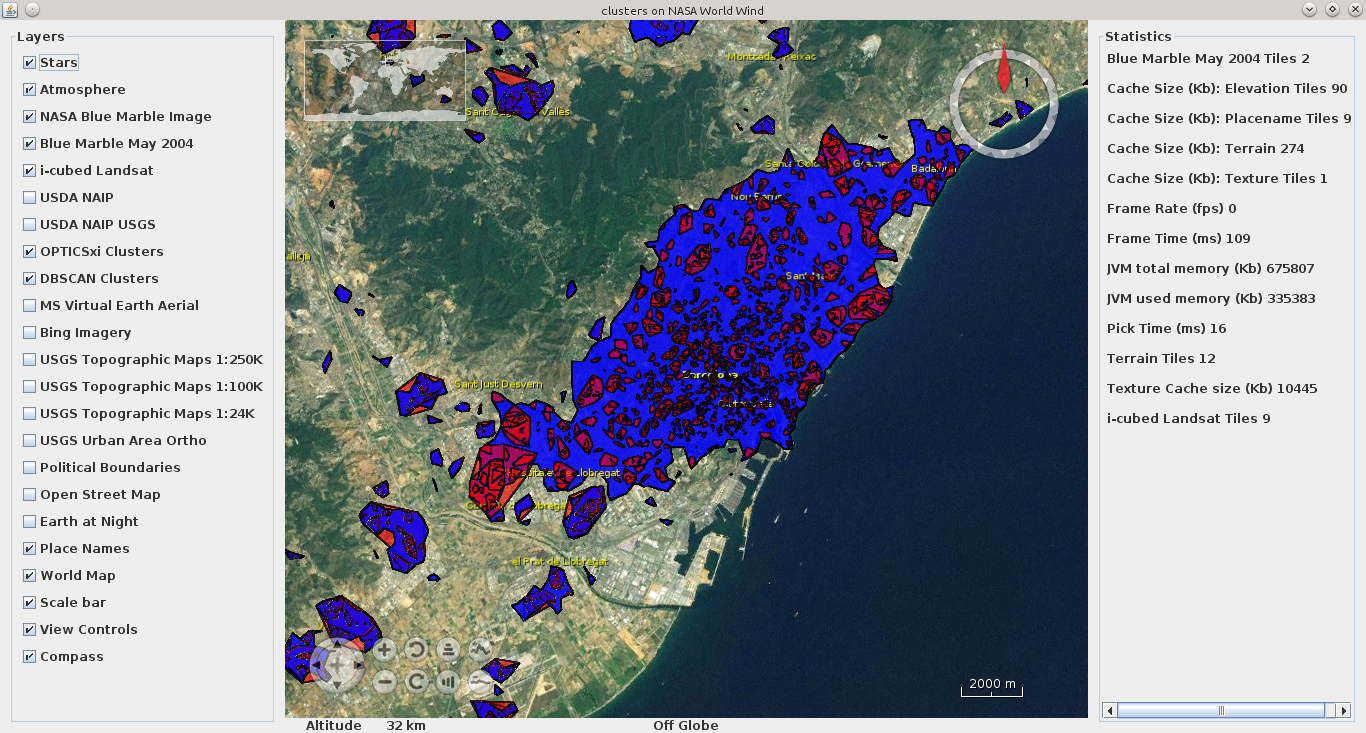
\includegraphics[width=0.4\textwidth]{screenshot1.png}\\
    \end{figure}         
    
\end{frame}

\begin{frame}
\frametitle{Clustering (cont.)}

    \begin{itemize}
      \item<1->In June 2014, it was released (the first?) QGIS plugin for \textit{spatially constrained clustering}: clusterpy.
      \begin{itemize}
	\item<1->\url{https://plugins.qgis.org/plugins/clusterpy\_qgis\_plugin/}
      \end{itemize}          
      \item<1->In this workshop we will use an alternative method to define areas with high density.
      \begin{itemize}
	\item<1->\url{http://www.qgistutorials.com/en/docs/creating_heatmaps.html}
      \end{itemize}          
    \end{itemize}    

    
\end{frame}


\begin{frame}
\frametitle{Hands-on}
\begin{itemize}
  \item<1->Objective: Detect areas with higher density of tweets.
  \item<1->Tool: QGIS.
  \item<1->Steps:  
  \begin{itemize}
    \item<2->Use the identify tool to establish a treshold; from that value on, pixels will be considered part of an high-density cluster.  
    \item<2->Use the raster calculator, to select pixels above that threshold (Raster$\rightarrow$Raster Calculator).
    \item<2->Example of a select expression:$"heatmap@1">150$    
    \item<3->The new map \textbf{only} contains binary values (1: above the threshold; 0: bellow the threshold).
    \item<3->Tip: ensure the legend picks up correctly the values on the dataset.
  \end{itemize}    
\end{itemize}  
\end{frame}

\begin{frame}
\frametitle{Hands-on (cont.)}
%\begin{itemize}
  \begin{itemize}
    \item<1->Vectorize this raster file (Raster$\rightarrow$Conversion$\rightarrow$Polygonize (Raster to Vector).  
    \item<2->Check out the attribute table of the Shapefile: verify the polygons have a value of 0, or 1 (right click + Open attribute table).
    \item<3->If we filter out the polygons with value 0, we will have the areas with high density. 
      \begin{itemize}
	\item<4->Select by expression: $"DN" = 1$. 
      \end{itemize}    
    \item<5->Save the selection as a new Shapefile.
    \item<6->Enhancement: count the number of tweets that fall within each polygon (Vector$\rightarrow$ Analysis Tools$\rightarrow$Count Points in Polygon).
    \item<7->Display the number of tweets within each polygon (right-click the layer to call the properties, and select "Labels").        
  \end{itemize}    
%\end{itemize}  
\end{frame}

\section{3D Viz} 
\begin{frame}
\frametitle{Three.js}
\begin{columns}
  \begin{column}{0.5\textwidth}\tiny{ 
  Lightweight cross-browser JavaScript library used to create and display animated 3D computer graphics on a Web browser.  
  \begin{itemize}
    \item<2->It relies on WebGL, a JavaScript API for rendering interactive 3D computer graphics and 2D graphics within any compatible web browser without the use of plug-ins.
    \item<3->WebGL itself is based on OpenGL ES 2.0, a subset of the OpenGL, an API for rendering hardware-accelerated graphics using a graphics processing unit (GPU).%visual processor unit (VPU), is a specialized electronic circuit designed to rapidly manipulate and alter memory to accelerate the creation of images in a frame buffer intended for output to a display.
\end{itemize}}
  \end{column}
  \begin{column}{0.5\textwidth}
      \begin{figure}  
	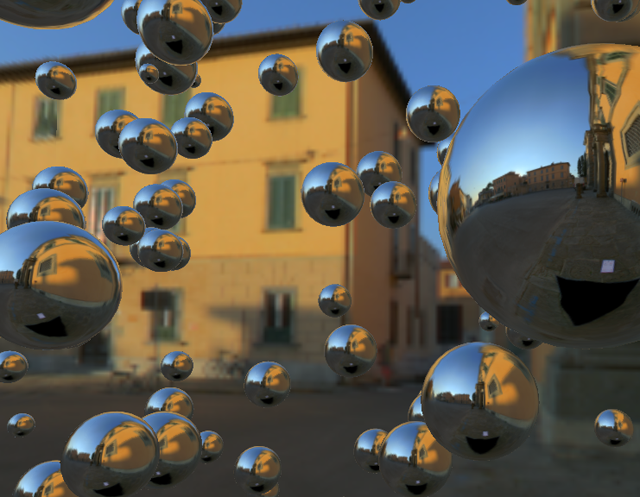
\includegraphics[width=\textwidth]{threejs2.png}    
      \end{figure}  
  \end{column}  
\end{columns}
\end{frame}

\begin{frame}
\frametitle{Three.js in QGGIS}
  \begin{itemize}
    \item<1->The Qgis2threejs plugin exports terrain data, map canvas image and vector data to a webpage.
    \item<2->The exported 3D objects can be viewed on any web browser which supports WebGL.%e.g.> chrome, firefox, ie, opera, ios
  \end{itemize}
    \begin{figure}  
      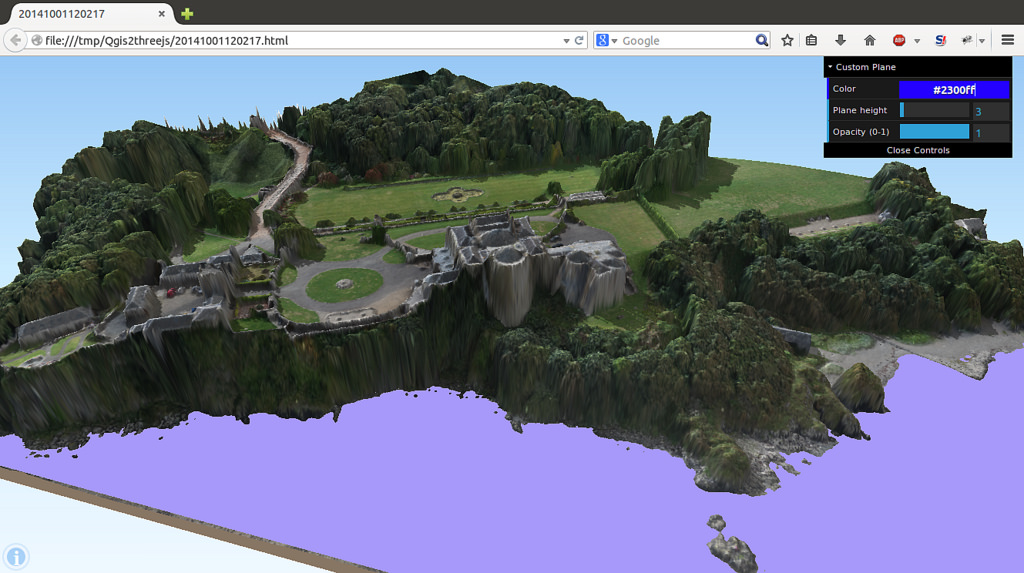
\includegraphics[width=0.6\textwidth]{3js.jpg}    
     \end{figure}  
\end{frame}

\begin{frame}
\frametitle{Hands-on}
\begin{itemize}
  \item<1->Objective: create webpage with 3d visualization of the clusters.
  \item<1->Tool: QGIS + Qgis2threejs plugin.
  \item<1->Steps:  
  \begin{itemize}
    \item<2->Ensure that Qgis2threejs is installed and enabled.  
    \item<3->Prepare the scene you want to render (e.g.: visible layers, styles, etc).
    \item<4->Run Qgis2threejs (Web$\rightarrow$Qgis2threejs$\rightarrow$Qgis2threejs)
    \item<5->Costumize the visualization. Some things to pay attention to:
      \begin{itemize}
	\item<6->Enable the layers you want to extrude (in this case, the clusters).      
	\item<6->The height value should be read from the count field (PNTCNT).	
	\item<6->You may want to exagerate the vertical scale by a factor.
	\item<6->The output HTML file path defines where you will save the result webpage (and associated files).	
      \end{itemize}    
    %\item<5->When you're ready, press the "run" button and wait for the visualization to come up.
  \end{itemize}    
\end{itemize}  
\end{frame}

%TODO: 3dviz intro, references + tutorials, fix _ character, fix images, review everything

\begin{frame}
\frametitle{Well Done!}
    \begin{figure}  
      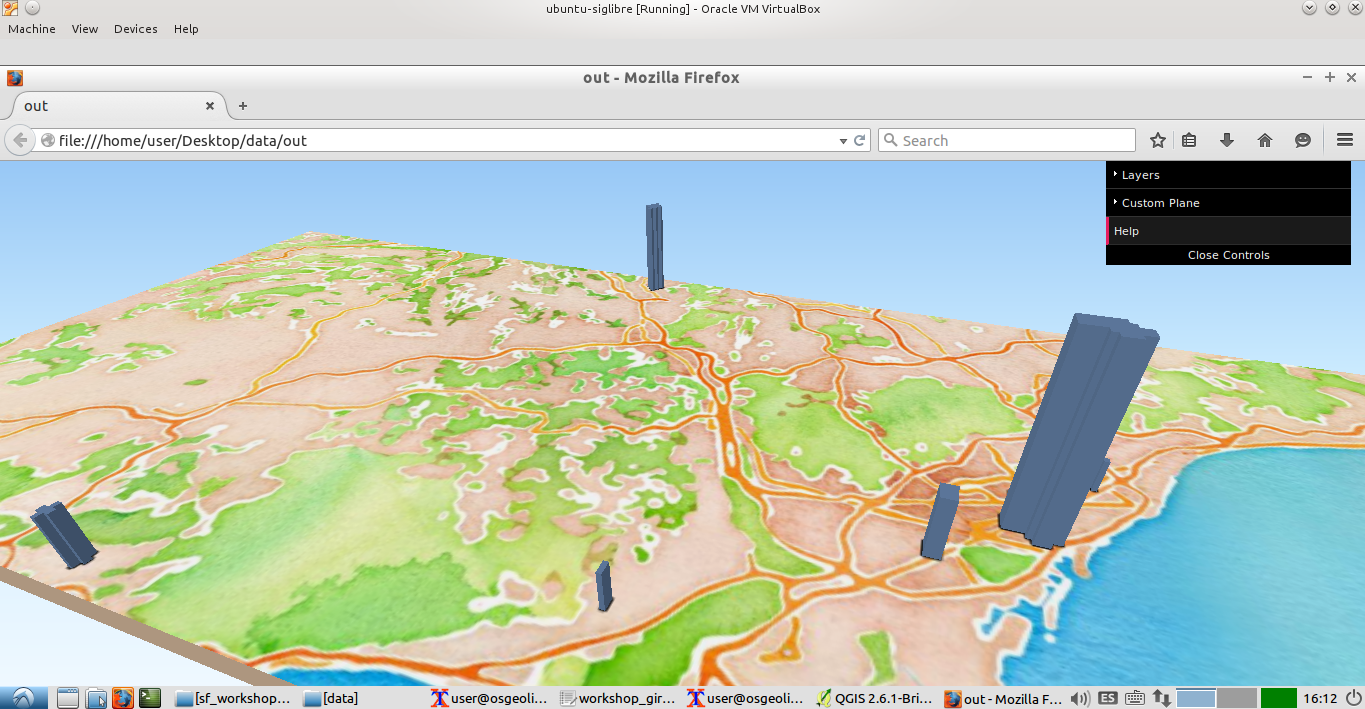
\includegraphics[width=\textwidth]{final.png}    
     \end{figure}  
\end{frame}


\begin{frame}
\frametitle{References}
\begin{itemize}\tiny{
\item \url{http://tweettracker.fulton.asu.edu/tda/TwitterDataAnalytics.pdf}
\item \url{http://www2.qgis.org}
\item \url{http://plugins.qgis.org/plugins/}
\item \url{http://geokoder.com/mongodb-plugin-for-quantum-gis}
\item \url{http://www.gislounge.com/heat-maps-in-gis/}
\item \url{https://alastaira.wordpress.com/2011/02/23/heat-mapping-crime-data-with-bing-maps-and-html5-canvas/}
\item \url{http://docs.qgis.org/2.0/en/docs/user_manual/plugins/plugins_heatmap.html}
\item \url{http://en.wikipedia.org/wiki/Kernel_\%28statistics\%29\#Kernel\_functions\_in\_common\_use}
\item \url{http://en.wikipedia.org/wiki/Cluster_analysis}
\item \url{https://plugins.qgis.org/plugins/clusterpy_qgis_plugin/}
\item \url{http://www.rise-group.org/section/Software/clusterPy/}
\item \url{http://threejs.org/}
\item \url{http://anitagraser.com/2014/03/15/3d-viz-with-qgis-three-js/} }
\end{itemize}
\end{frame}

\

\end{document}